\subsubsection{Analisis termico}
\FloatBarrier

Por el transistor de paso, en el peor de los casos, va a tener una caída de $V_{SD} = V_{CC} - V_O = 9.5V - 5V = 4.5V$, y va a circular una corriente máxima de $I_{L} = 1.5A$, llegando a tener una $P_{C,MAX} = \SI{6.75}{\watt}$. Por ende es necesario realizar un análisis térmico y ver si requiere agregar un disipador en dicho transistor de paso:

Los siguientes datos fueron obtenidos del datasheet y de nuestro circuito:
\begin{multicols}{2}
\begin{itemize}
    \item $R_{jc} = \SI{0.75}{\celsius\per\watt}$
    \item $R_{cs} = \SI{0.5}{\celsius\per\watt}$
    \item $R_{ja} = \SI{62}{\celsius\per\watt}$
    \item $T_a = \SI{50}{\celsius}$
    \item $T_{j,\text{MAX}} = \SI{175}{\celsius}$
    \item $P_{c,\text{MAX}} = \SI{6.75}{\watt}$
\end{itemize}
\end{multicols}

\begin{figure}[h]
    \centering
    
    \begin{minipage}{0.48\textwidth}
        \centering
        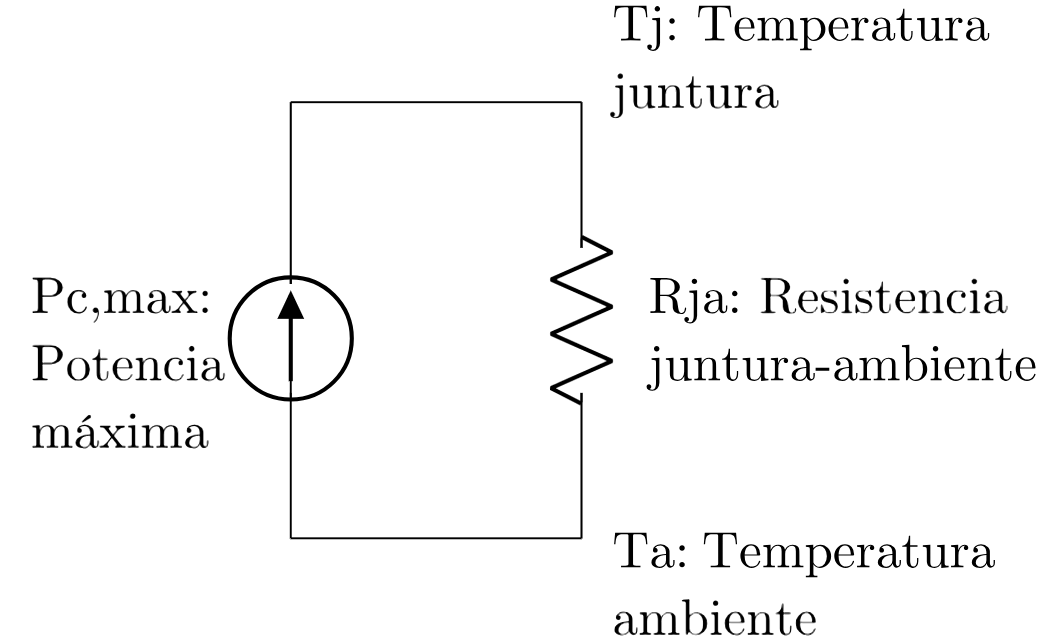
\includegraphics[width=\textwidth]{img/analisis_termico/circuito_termico_sin_rsa.png}
        \caption{Modelo térmico sin $R_{sa}$}
        \label{fig:circuito_termico_sin_rsa}
    \end{minipage}
    \hfill
    \begin{minipage}{0.48\textwidth}
        Primero se analizamos si la temperatura máxima que llega $T_j$, sin el disipador, supera a la temperatura de juntura máxima permitida:
        \begin{align*}
            T_{j} &= T_{ja} + T_{a} \\
            T_{j} &= P_{C,MAX} \cdot R_{ja} + T_{a} \\
            T_{j} &= \SI{419}{\celsius} + \SI{50}{\celsius} \\
            T_{j} &= \SI{469}{\celsius}
        \end{align*}
        \begin{align}
            \boxed{T_{j} = \SI{469}{\celsius} \gg T_{j,MAX} = \SI{175}{\celsius}}
        \end{align}
        Se observa que si no hay un disipador, la temperatura de la juntura supera la máxima permitida.
    \end{minipage}

\end{figure}


Ahora se analiza que $R_{sa}$ máxima es necesaria tal que la temperatura de juntura no supere la máxima permitida.
\begin{figure}[h]
    \centering
    
    \begin{minipage}{0.48\textwidth}
        \centering
        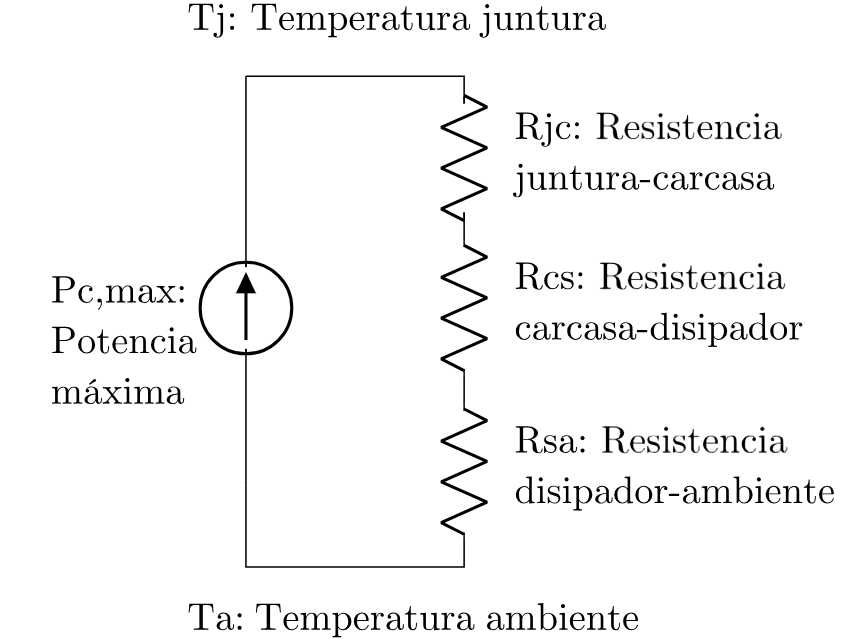
\includegraphics[width=\textwidth]{img/analisis_termico/circuito_termico_con_rsa.png}
        \caption{Modelo térmico con $R_{sa}$}
        \label{fig:circuito_termico_con_rsa}
    \end{minipage}
    \hfill
    \begin{minipage}{0.48\textwidth}
        \begin{align*}
            R_{total} &=  R_{jc} + R_{cs} + R_{sa,MAX} \\
            \dfrac{T_{j,MAX} - T_a }{P_{C,MAX}} &=  R_{jc} + R_{cs} + R_{sa,MAX} \\
            R_{sa,MAX} &= \dfrac{T_{j,MAX} - T_a }{P_{C,MAX}} - R_{jc} - R_{cs} \\
            R_{sa,MAX} &= \SI{17.3}{\celsius\per\watt}
        \end{align*}
        \begin{align}
            \boxed{R_{sa} \le R_{sa,MAX} = \SI{17.3}{\celsius\per\watt}}
        \end{align}
        Se debe elegir un disipador con un $R_{sa}$ que cumpla esta condicion para que el transistor de paso no se queme.
    \end{minipage}

\end{figure}


Se elige el siguiente disipador:

\begin{figure}[h]
    \centering
    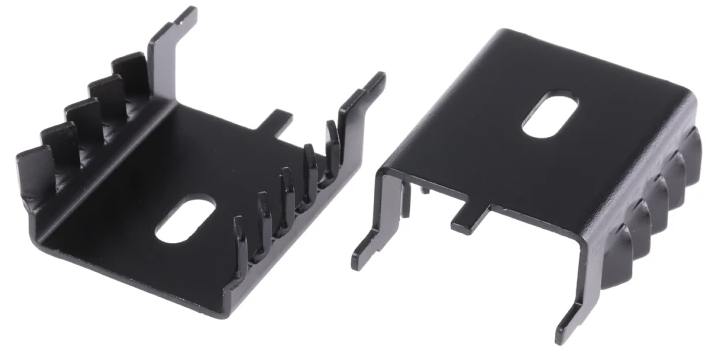
\includegraphics[width=0.5\textwidth]{img/analisis_termico/disipador.png}
    \caption{Disipador}
    \label{fig:disipador}
\end{figure}

Se selecciona un disipador del fabricante AAVID Thermalloy, diseñado para encapsulados tipo TO-220. Este disipador presenta dimensiones (35 mm × 12.3 mm × 29 mm).

La elección de este disipador se justifica debido a que su resistencia térmica cumple con la condición de diseño requerida:
\begin{align}
    \boxed{R_{sa} = \SI{13}{\celsius\per\watt} < R_{sa,MAX} = \SI{17.3}{\celsius\per\watt}}
\end{align}

Por lo tanto, el dispositivo garantiza que la temperatura de juntura del transistor se mantenga dentro de los límites seguros de operación.

\FloatBarrier

